%% ============================================================
%%  Memoria Práctica 2 – Arquitectura de Computadores
%%  Método de Jacobi: Multinúcleo y extensiones SIMD
%%  Compilar con: lualatex memoria.tex  (2 pasadas)
%% ============================================================
\documentclass[a4paper,twocolumn]{article}

%% ── Fuentes (LuaLaTeX/MiKTeX) ──────────────────────────────
%% ORDEN CRÍTICO: babel ANTES que fontspec en LuaLaTeX
\usepackage[spanish]{babel}
\usepackage{fontspec}
\defaultfontfeatures{Ligatures=TeX}
%% TeX Gyre Pagella cargada por nombre de fichero (no requiere instalación
%% separada: viene con MiKTeX en el paquete tex-gyre).
%% Si sigue fallando, instala el paquete "tex-gyre" desde MiKTeX Console
%% o descomenta la línea con Latin Modern:
%\setmainfont{Latin Modern Roman}
\setmainfont[
  UprightFont    = *-regular,
  BoldFont       = *-bold,
  ItalicFont     = *-italic,
  BoldItalicFont = *-bolditalic
]{texgyrepagella}
\linespread{1.05}
\usepackage{microtype}

%% ── Matemáticas ─────────────────────────────────────────────
\usepackage{amsmath, amssymb}

%% ── Geometría ───────────────────────────────────────────────
\usepackage[hmarginratio=1:1, top=28mm, bottom=22mm,
            left=18mm, right=18mm, columnsep=18pt]{geometry}

%% ── Figuras / tablas ────────────────────────────────────────
\usepackage{graphicx}
\usepackage{booktabs}
\usepackage[hang,small,labelfont=bf,up,textfont=it,up]{caption}
\usepackage{float}

%% ── Listas ──────────────────────────────────────────────────
\usepackage{enumitem}
\setlist[itemize]{noitemsep, topsep=2pt}
\setlist[enumerate]{noitemsep, topsep=2pt}

%% ── Código fuente ───────────────────────────────────────────
\usepackage{listings}
\usepackage{xcolor}
\definecolor{codebg}{HTML}{F5F5FA}
\definecolor{kwcol}{HTML}{0057AE}
\definecolor{cmcol}{HTML}{777788}
\lstset{
  language=C,
  backgroundcolor=\color{codebg},
  frame=single, rulecolor=\color{gray!35},
  basicstyle=\ttfamily\scriptsize,
  keywordstyle=\color{kwcol}\bfseries,
  commentstyle=\color{cmcol}\itshape,
  numbers=none,
  breaklines=true,
  xleftmargin=3pt, xrightmargin=3pt,
  aboveskip=4pt, belowskip=4pt
}

%% ── Abstract ────────────────────────────────────────────────
\usepackage{abstract}
\renewcommand{\abstractnamefont}{\normalfont\bfseries}
\renewcommand{\abstracttextfont}{\normalfont\small\itshape}

%% ── Secciones (igual que plantilla) ────────────────────────
\usepackage{titlesec}
\renewcommand\thesection{\Roman{section}}
\renewcommand\thesubsection{\Alph{subsection}}
\titleformat{\section}[block]{\large\scshape\centering}{\thesection.}{1em}{}
\titleformat{\subsection}[block]{\normalsize\bfseries}{\thesubsection.}{0.8em}{}
\titlespacing*{\section}{0pt}{8pt}{4pt}
\titlespacing*{\subsection}{0pt}{5pt}{2pt}

%% ── Cabecera / pie ──────────────────────────────────────────
\usepackage{fancyhdr}
\pagestyle{fancy}
\fancyhead{}\fancyfoot{}
\fancyhead[C]{\small\itshape Práctica 2 AC --- Jacobi multinúcleo y SIMD}
\fancyfoot[C]{\thepage}
\renewcommand{\headrulewidth}{0.4pt}

%% ── Hipervínculos ───────────────────────────────────────────
\usepackage{hyperref}
\hypersetup{colorlinks=true, linkcolor=black, citecolor=black, urlcolor=blue,
            pdftitle={Memoria Practica 2 AC}, pdfauthor={Alvaro Schwiedop}}

%% ── Título ──────────────────────────────────────────────────
\usepackage{titling}
\setlength{\droptitle}{-4\baselineskip}
\pretitle{\begin{center}\LARGE\bfseries}
\posttitle{\end{center}\vspace{-4pt}}

\title{Programación Multinúcleo y Extensiones SIMD:\\[4pt]
       Implementación y Análisis del Método de Jacobi}

\author{%
  \textsc{Baptiste Robin, Álvaro Schwiedop Souto}\\[0.5ex]
  \normalsize Arquitectura de Computadores \textbullet{} 2\textordmasculine{} Grao Enx. Informática\\
  \normalsize Universidade de Santiago de Compostela\\
  \normalsize \texttt{curso1523@usc.es}
}
\date{\today}

\renewcommand{\maketitlehookd}{%
  \begin{abstract}
    \noindent
    Se implementan cuatro versiones del método iterativo de Jacobi en C sobre el
    supercomputador FinisTerrae~III del CESGA: versión secuencial de referencia
    (v1), versión optimizada para caché con división de lazos, desenrollamiento
    y \textit{blocking} (v2), versión paralela con OpenMP (v3) y versión
    vectorial con instrucciones AVX256 y FMA (v4).
    % AUTO_ABSTRACT_RESULTS_BEGIN
    La actualización automática de resultados insertará aquí el resumen cuantitativo
    principal a partir de los ficheros de \texttt{resultados/}.\\[2pt]
    % AUTO_ABSTRACT_RESULTS_END
    \textbf{\textit{Palabras clave}:} Jacobi, AVX256, FMA, OpenMP,
    \textit{cache blocking}, \textit{speedup}, FinisTerrae~III.
  \end{abstract}
}

%% ============================================================
\begin{document}
\maketitle

%%=============================================================
\section{Introducción}

El método de Jacobi~\cite{saad2003} es un algoritmo iterativo clásico para la
resolución de sistemas $Ax{=}b$ con matriz diagonalmente dominante.  Partiendo de
$x^{(0)}{=}\mathbf{0}$, en cada iteración se actualiza:
\[
  x_i^{(k+1)} = \frac{1}{a_{ii}}\!\left(b_i - \sum_{j \neq i} a_{ij}\,x_j^{(k)}\right)
\]
hasta que $\|x^{(k+1)}-x^{(k)}\|_2 < \text{tol}$.  La doble suma implica
$\mathcal{O}(n^2)$ operaciones por iteración, lo que hace que tamaños grandes
sean costosos y susceptibles de aceleración mediante optimizaciones de bajo nivel.

El objetivo es implementar cuatro versiones de complejidad creciente, medirlas en
FinisTerrae~III (Intel Xeon Platinum 8352Y, 2.2~GHz, 64~núcleos por nodo) y
cuantificar el \textit{speedup} obtenido.  La Sección~II describe las
implementaciones; la Sección~III, la metodología experimental; la Sección~IV,
los resultados; la Sección~V, las conclusiones.

%%=============================================================
\section{Implementaciones}

\subsection{v1 --- Secuencial base}

Traducción directa del pseudocódigo del enunciado sin ninguna
optimización manual. El algoritmo recibe la matriz $A$, el vector
$b$, la tolerancia \texttt{tol} y el máximo de iteraciones
\texttt{max\_iter}; itera actualizando $x$ hasta convergencia:

\begin{center}
\small
\begin{tabular}{l}
\hline
\textbf{Entradas:} $A\in\mathbb{R}^{n\times n}$, $b,x\in\mathbb{R}^n$,
  \texttt{tol}, \texttt{max\_iter}\\
\textbf{Aux:} $x\_new\in\mathbb{R}^n$\\
\hline
\textbf{para} $\mathit{iter}=0$ \textbf{hasta} $\mathit{max\_iter}$:\\
\quad $\mathit{norm2} \leftarrow 0$\\
\quad \textbf{para} $i=0$ \textbf{hasta} $n-1$:\\
\quad\quad $\sigma \leftarrow 0$\\
\quad\quad \textbf{para} $j=0$ \textbf{hasta} $n-1$:\\
\quad\quad\quad \textbf{si} $i \neq j$: $\;\sigma \mathrel{+}= a[i][j]\cdot x[j]$\\
\quad\quad $x\_new[i] \leftarrow (b[i]-\sigma)\,/\,a[i][i]$\\
\quad\quad $\mathit{norm2} \mathrel{+}= (x\_new[i]-x[i])^2$\\
\quad $x \leftarrow x\_new$\\
\quad \textbf{si} $\sqrt{\mathit{norm2}} < \mathit{tol}$: \textbf{terminar}\\
\textbf{Salida:} imprimir $\mathit{norm2}$\\
\hline
\end{tabular}
\end{center}

La implementación en C introduce la condición \texttt{if(i!=j)}
dentro del bucle interno, lo cual genera una rama innecesaria:

\begin{lstlisting}
for (int j = 0; j < n; j++)
  if (i != j)
    sigma += a[i*n+j] * x[j];
x_new[i] = (b[i]-sigma) / a[i*n+i];
\end{lstlisting}

Se usa como referencia de rendimiento y corrección numérica.

\subsection{v2 --- Optimizaciones de caché}

Se aplican cuatro mejoras sobre v1:

\begin{enumerate}
  \item \textbf{Reducción de instrucciones:} puntero de fila
        \texttt{const double *row=\&a[i*n]}, elimina el recalculo del índice.
  \item \textbf{División de lazos:} el bucle \texttt{j} se parte en
        $[0,i)$ e $(i,n)$, eliminando la rama condicional.
  \item \textbf{Desenrollamiento $\times$4:} cuatro acumulaciones explícitas
        por iteración.
  \item \textbf{\textit{Cache blocking}:} bloques de \texttt{BLOCK\_SIZE=64}
        filas para mantener $x$ en caché L1/L2.
\end{enumerate}

\subsection{v3 --- OpenMP}

La región \texttt{parallel} se sitúa \textit{fuera} del bucle de
iteraciones para mantener vivos los hilos entre iteraciones y evitar
\textit{fork/join} repetido.  La variante base usa
\texttt{reduction(+:norm2)} con \texttt{schedule(static)} y, a partir del mismo
fuente, se compilan las variantes \texttt{dynamic(16)}, \texttt{guided} y
\texttt{critical}.  La sincronización entre iteraciones se realiza mediante
barreras implícitas y un bloque \texttt{omp single}:

\begin{lstlisting}
#pragma omp parallel default(none) \
    shared(a,b,x,x_new,n,norm2,...)
{
  while (...) {
    #pragma omp for schedule(static) \
        reduction(+:norm2)
    for (int i=0; i<n; i++) { ... }
    #pragma omp single
    { converged = sqrt(norm2) < tol; iter++; }
    #pragma omp for schedule(static)
    for (int i=0; i<n; i++) x[i] = x_new[i];
  }
}
\end{lstlisting}

\subsection{v4 --- AVX256 + FMA}

Se emplea \texttt{\_\_m256d} (4~\texttt{double}/registro) con
\texttt{\_mm256\_fmadd\_pd}.  La memoria se reserva alineada a 32~B con
\texttt{aligned\_alloc} y el \textit{stride} de fila se redondea a múltiplo
de~4 (\texttt{n\_pad}).  La reducción horizontal usa \texttt{\_mm256\_hadd\_pd}:

\begin{lstlisting}
__m256d va = _mm256_load_pd(&row[j]);
__m256d vx = _mm256_load_pd(&x[j]);
vsigma = _mm256_fmadd_pd(va, vx, vsigma);
/* reduccion horizontal al final */
__m256d h = _mm256_hadd_pd(vsigma, vsigma);
\end{lstlisting}

No se usan intrínsecos \texttt{\_u} (no alineados) como exige el enunciado.

%%=============================================================
\section{Metodología experimental}

Los experimentos se ejecutan en FinisTerrae~III mediante trabajos SLURM en la
partición \texttt{short}.  El tiempo se mide en \textbf{ciclos de reloj} con
\texttt{get\_counter()} basada en el TSC, englobando sólo el cómputo iterativo.
Para cada configuración se toman \textbf{10 medidas independientes} y se
selecciona la \textbf{mediana} para reducir perturbaciones del SO.

Parámetros fijos: $\text{tol}{=}10^{-5}$, $\text{max\_iter}{=}15000$,
$\texttt{srand}(42)$, dominancia diagonal garantizada sumando la suma de fila
al elemento diagonal.  Niveles de optimización: \texttt{-O0} y \texttt{-O3};
v3 usa \texttt{-fopenmp}; v4 añade \mbox{\texttt{-mavx2 -mfma}}.  Hilos evaluados:
$\{1,2,4,8,16,32\}$.

La Tabla~\ref{tab:medianas} resume las medianas obtenidas.

\begin{table}[tb]
{\footnotesize
\caption{Medianas de ciclos ($\times 10^9$) por versión y tamaño}
\label{tab:medianas}
\centering
\setlength{\tabcolsep}{5pt}
\begin{tabular}{lrrr}
\toprule
\textbf{Versión} & $n{=}1250$ & $n{=}2000$ & $n{=}3200$ \\
\midrule
% AUTO_TABLE_ROWS_BEGIN
v1 \texttt{-O0}       & 57.5 & 221.8 & 901.2 \\
v1 \texttt{-O3}       & 26.4 & 105.9 & 425.0 \\
v2 \texttt{-O0}       & 58.4 & 222.3 & 895.2 \\
v2 \texttt{-O3}       & 26.5 &  99.8 & 400.9 \\
v4 \texttt{-O0}       & 42.1 & 162.0 & 661.9 \\
v4 \texttt{-O3}       & 14.8 &  65.8 & 272.9 \\
v3 \texttt{-O3} (1T)  & 24.4 &  96.6 & 395.9 \\
v3 \texttt{-O3} (32T) &  2.4 &   4.8 &  18.7 \\
% AUTO_TABLE_ROWS_END
\bottomrule
\end{tabular}
}
\end{table}

%%=============================================================
\section{Resultados y análisis}

\subsection{Efecto de las optimizaciones de caché}

% AUTO_G1_TEXT_BEGIN
La Figura~\ref{fig:g1} muestra el \textit{speedup} de v2 respecto a v1 con ambas
versiones en \texttt{-O0}.  Este bloque se sustituirá automáticamente con la
interpretación cuantitativa calculada desde \texttt{resultados/}.
% AUTO_G1_TEXT_END

\begin{figure}[H]
  \centering
  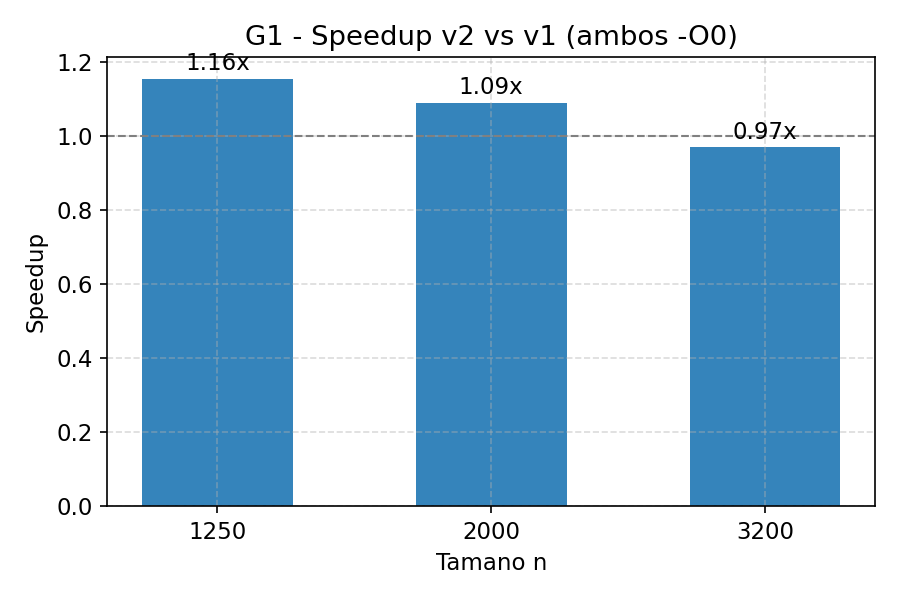
\includegraphics[width=\linewidth]{graficas/g1_speedup_v2_vs_v1_O0.png}
  \caption{Speedup v2/v1 con \texttt{-O0}.}
  \label{fig:g1}
\end{figure}

\subsection{Todas las versiones vs.\ v1-O3}

% AUTO_G2_TEXT_BEGIN
La Figura~\ref{fig:g2} compara la versión secuencial optimizada (v2), la mejor
configuración OpenMP (v3) y la versión SIMD (v4) respecto a v1\texttt{-O3}.
Este bloque será sustituido automáticamente con la interpretación cuantitativa
obtenida a partir de los ficheros de resultados.
% AUTO_G2_TEXT_END

\begin{figure}[H]
  \centering
  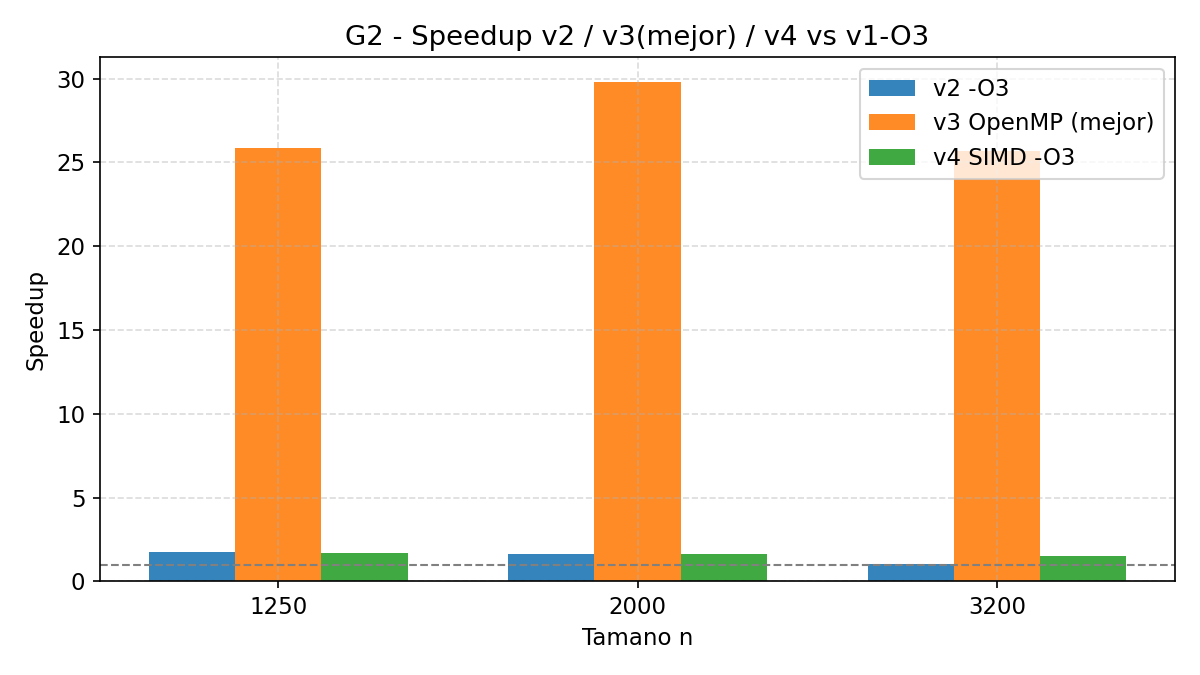
\includegraphics[width=\linewidth]{graficas/g2_speedup_vs_v1O3.png}
  \caption{Speedup de v2\texttt{-O3}, la mejor configuración de v3 y
           v4\texttt{-O3} respecto a v1\texttt{-O3}.}
  \label{fig:g2}
\end{figure}

\subsection{v3 y v4 vs.\ v2-O3}

% AUTO_G3_TEXT_BEGIN
La Figura~\ref{fig:g3} muestra el \textit{speedup} de la mejor configuración
OpenMP (v3) y de la versión SIMD (v4) respecto a v2\texttt{-O3}.  Este bloque
será sustituido automáticamente con los valores calculados desde
\texttt{resultados/}.
% AUTO_G3_TEXT_END

\begin{figure}[H]
  \centering
  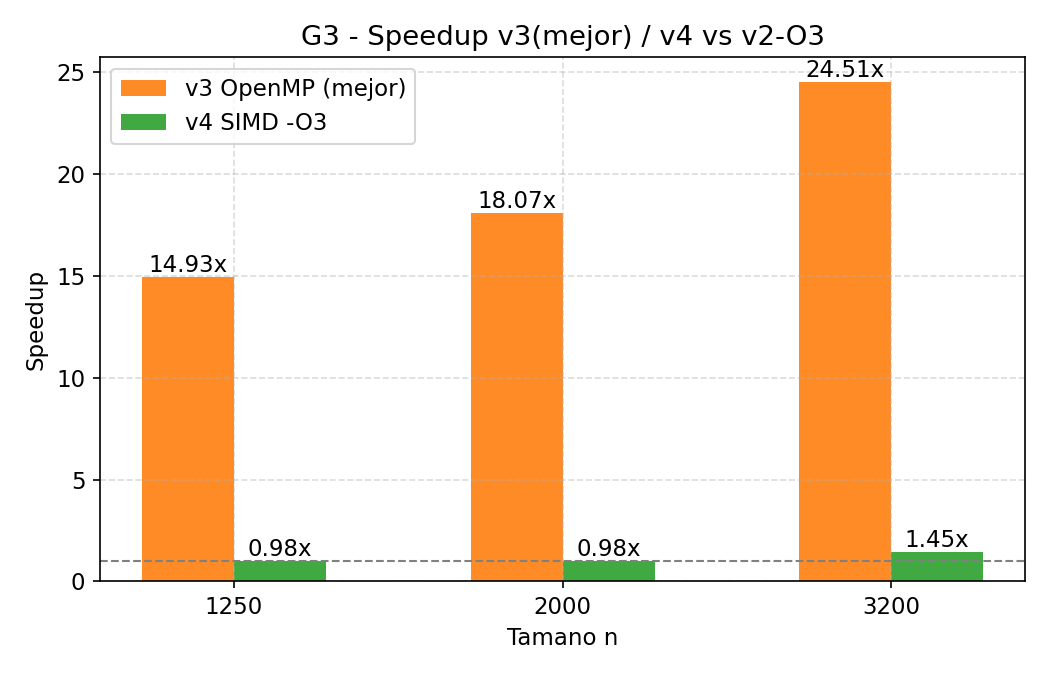
\includegraphics[width=\linewidth]{graficas/g3_speedup_v3_v4_vs_v2O3.png}
  \caption{Speedup de la mejor configuración de v3 y de v4\texttt{-O3}
           respecto a v2\texttt{-O3}.}
  \label{fig:g3}
\end{figure}

\subsection{Escalabilidad de v3 con el número de hilos}

% AUTO_G4_TEXT_BEGIN
La Figura~\ref{fig:g4} es la gráfica \textbf{obligatoria} del enunciado y
resume el speedup de v3\texttt{-O3} con \texttt{schedule(static)} frente a su
ejecución con un hilo.  Este bloque se sustituirá automáticamente con el
análisis cuantitativo de los resultados medidos.
% AUTO_G4_TEXT_END

\begin{figure}[H]
  \centering
  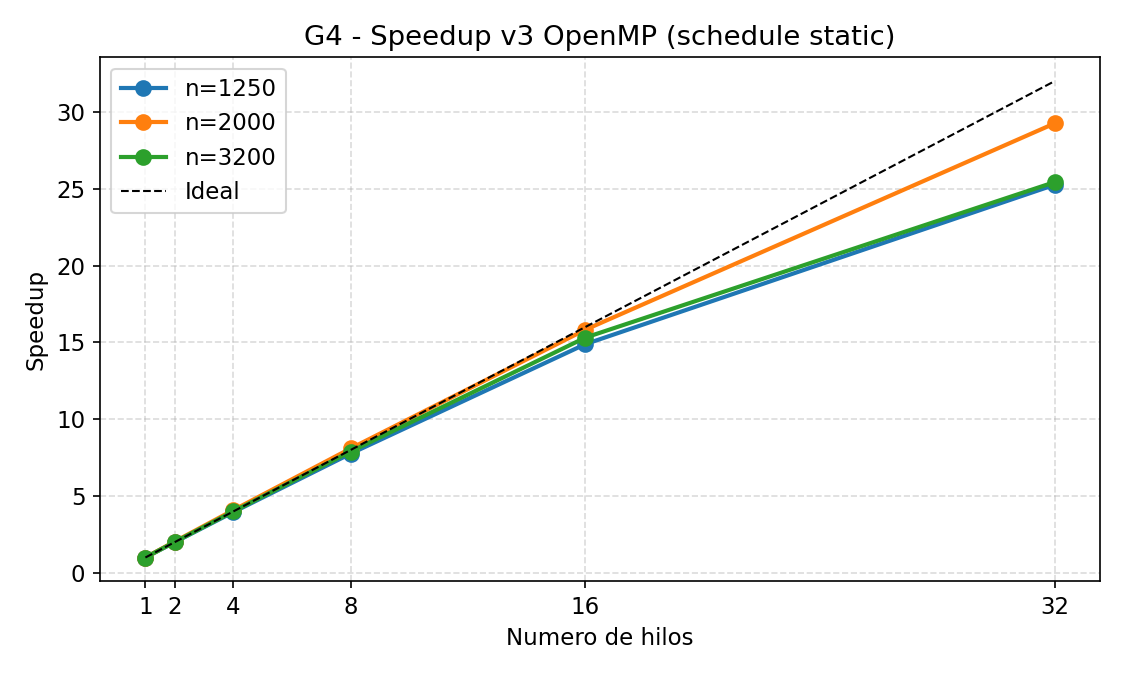
\includegraphics[width=\linewidth]{graficas/g4_speedup_hilos.png}
  \caption{Speedup de v3\texttt{-O3} (\texttt{schedule(static)}) frente a
           1~hilo para cada $n$.  Línea discontinua: ideal lineal.}
  \label{fig:g4}
\end{figure}

\subsection{Comparación de schedulings}

% AUTO_G5_TEXT_BEGIN
La Figura~\ref{fig:g5} compara los tres modos de reparto de OpenMP sobre v3.
Este bloque se sustituirá automáticamente con el resumen numérico de la mejor
política para cada tamaño.
% AUTO_G5_TEXT_END

\begin{figure*}[h]
  \vspace{-4pt}
  \centering
  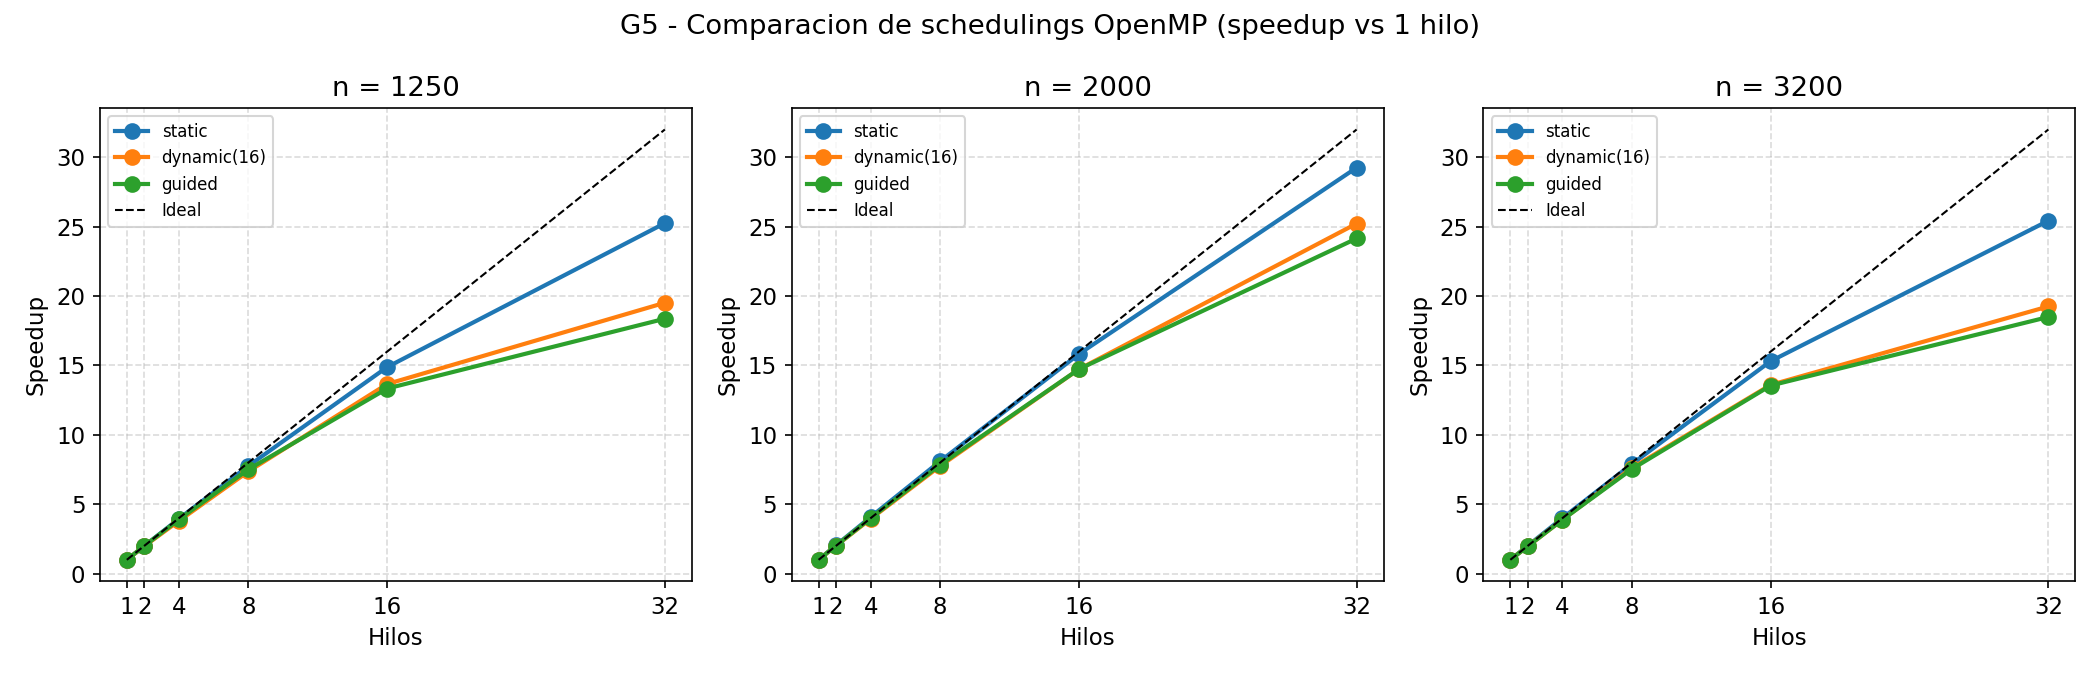
\includegraphics[width=0.96\textwidth]{graficas/g5_schedulings.png}
  \caption{Comparación de schedulings OpenMP para v3 y
           $n\in\{1250,2000,3200\}$.}
  \label{fig:g5}
\end{figure*}

\subsection{Reducción reduction vs.\ critical}

% AUTO_G6_TEXT_BEGIN
La Figura~\ref{fig:g6} compara la variante base con
\texttt{reduction(+:norm2)} frente a la variante con \texttt{critical}.  Este
bloque se sustituirá automáticamente con el análisis cuantitativo extraído de
los ficheros de resultados.
% AUTO_G6_TEXT_END

\begin{figure*}[h]
  \vspace{-4pt}
  \centering
  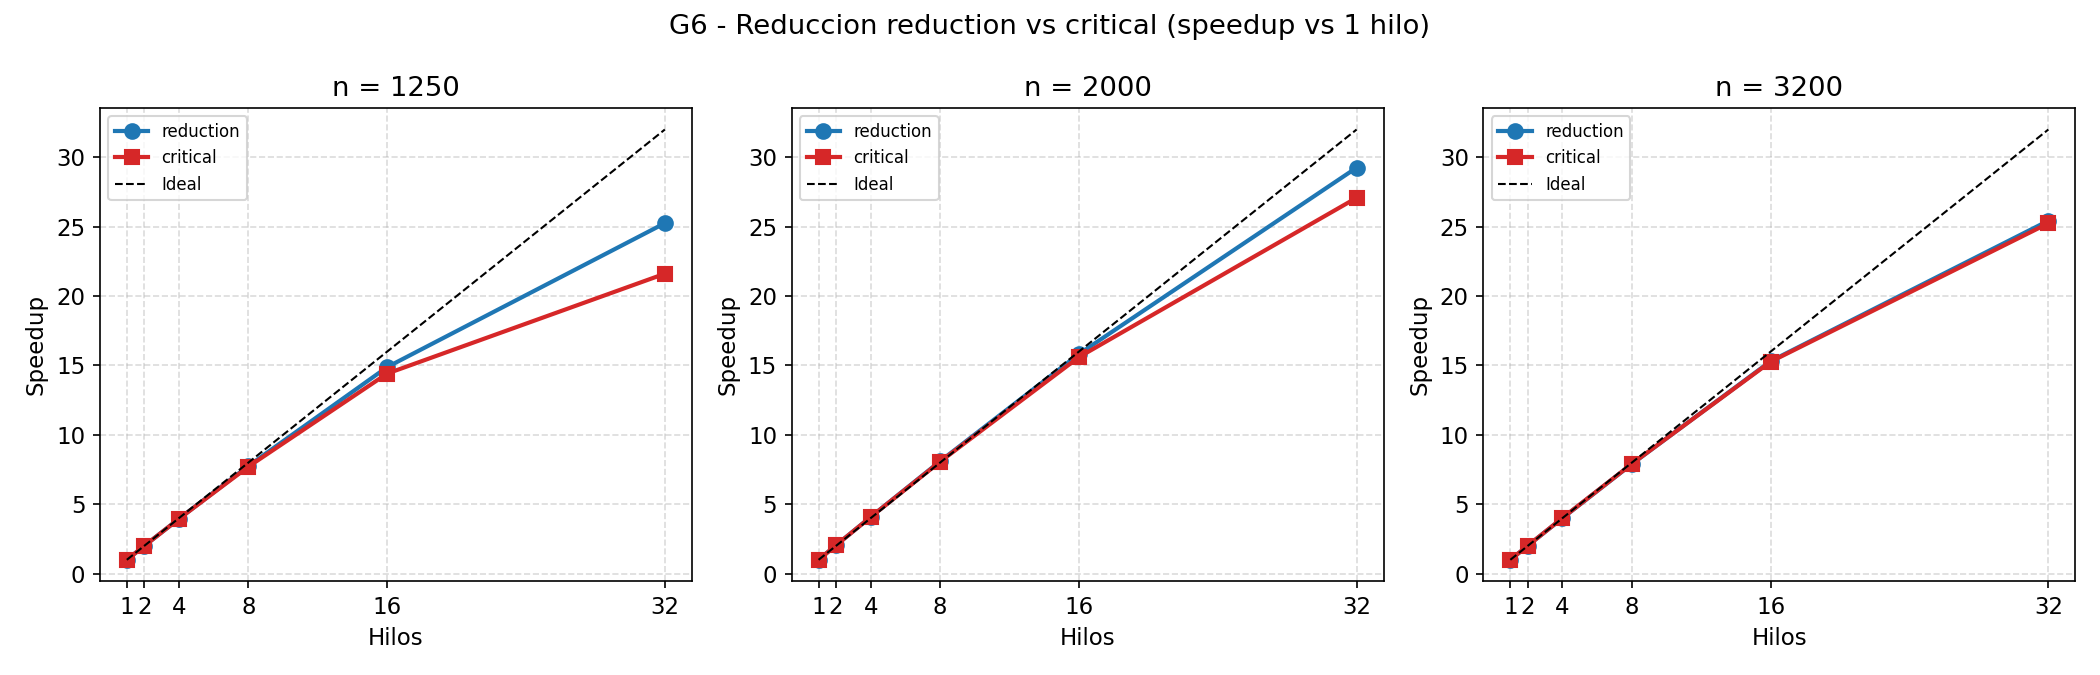
\includegraphics[width=0.96\textwidth]{graficas/g6_atomic_vs_critical.png}
  \caption{Comparación de reducción \texttt{reduction} vs.\ \texttt{critical}
           en v3.}
  \label{fig:g6}
\end{figure*}

%%=============================================================
\section{Conclusiones}

% AUTO_CONCLUSIONS_BEGIN
Se han implementado y evaluado cuatro versiones del método de Jacobi.  Este
bloque se sustituirá automáticamente con las conclusiones cuantitativas
extraídas de los ficheros de resultados.
% AUTO_CONCLUSIONS_END

Como trabajo futuro se propone combinar v3 y v4 (SIMD+OpenMP) y estudiar el
impacto del \textit{thread binding} (\texttt{OMP\_PROC\_BIND}) sobre la coherencia
de caché en entornos NUMA.

%%=============================================================
\begin{thebibliography}{9}

\bibitem{saad2003}
  Y.~Saad,
  \textit{Iterative Methods for Sparse Linear Systems}, 2nd~ed.
  SIAM, Philadelphia, 2003.

\bibitem{intel_intrinsics}
  Intel Corporation,
  \textit{Intel Intrinsics Guide},
  \url{https://www.intel.com/content/www/us/en/docs/intrinsics-guide/},
  \newblock [online] última visita marzo 2026.

\bibitem{openmp30}
  OpenMP Architecture Review Board,
  \textit{OpenMP API v3.0 Summary Spec},
  \url{https://www.openmp.org/wp-content/uploads/OpenMP3.0-SummarySpec.pdf},
  noviembre 2008.

\bibitem{patterson}
  D.~A.~Patterson y J.~L.~Hennessy,
  \textit{Computer Organization and Design}, 5th~ed.
  Morgan Kaufmann, 2014.

\end{thebibliography}

\end{document}
